\chapter{Introducción}\label{chapter:introduction}
\addcontentsline{toc}{chapter}{Introducción}

La medicina moderna ha fortalecido el control de enfermedades mediante el desarrollo de vacunas. 
Sin embargo, su aplicación masiva en la población exige garantizar su seguridad de manera rigurosa y continua.
Esta exigencia toma forma en un proceso escalonado de investigación clínica, que transcurre por diversas etapas antes de la aprobación del fármaco, tal como ilustra la figura \ref{fig:desarrollo_clinico}.

En las etapas I, II y III, el producto atraviesa estudios controlados en grupos seleccionados de voluntarios para reunir datos preliminares sobre su seguridad y definir las recomendaciones de posología y eficacia a corto plazo. 
Durante estas fases, el producto biológico permanece en un entorno científico resguardado, donde la población de estudio es reducida (rara vez superando los 5,000 sujetos) y generalmente homogénea, lo que limita la detección de reacciones poco frecuentes \cite{who_pharmacovigilance_2004}.

\begin{figure}[htbp]
    \centering
    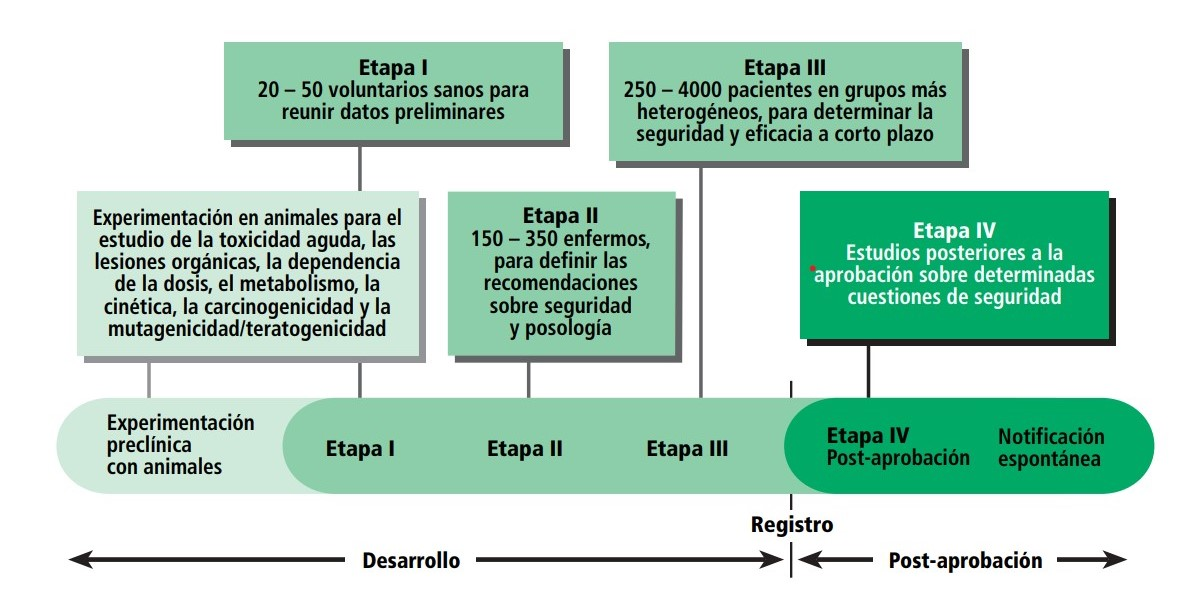
\includegraphics[width=0.8\textwidth]{Graphics/Cap1/fig1_desarrollo_clinico.jpg}
    \caption{Etapas del desarrollo clínico de vacunas. Adaptado de \cite{who_pharmacovigilance_2004}.}
    \label{fig:desarrollo_clinico}
\end{figure}

Una vez que la \gls{vacuna} recibe el registro sanitario y comienza su uso masivo en la población general, inicia la etapa IV o post-aprobación. 
En estas condiciones reales de uso, el escenario cambia drásticamente: el producto alcanza a grupos diversos que incluyen niños, ancianos, embarazadas y personas con múltiples patologías, quienes a menudo fueron excluidos de los ensayos iniciales \cite{who_pharmacovigilance_2004}.

Precisamente en esta fase es donde comienzan a manifestarse los eventos supuestamente atribuibles a la vacunación o inmunización (ESAVI), definidos como cualquier cuadro clínico desfavorable (signo, síntoma o enfermedad) que ocurre tras la vacunación y no necesariamente tiene una relación causal con la vacuna \cite{paho_curso_esavi}.

Para gestionar estos riesgos inevitables, surge la \gls{farmacovigilancia} como la ciencia y las actividades relativas a la detección, evaluación, comprensión y prevención de los efectos adversos de los medicamentos.
Esta disciplina permite evaluar continuamente la relación beneficio-riesgo y detectar señales de alerta que no fueron identificadas durante las fases iniciales de investigación \cite{who_pharmacovigilance_2004}.

\section{Contexto histórico y social de la farmacovigilancia}\label{section:contextoHistoricoSocial}

La evolución de la farmacovigilancia ha estado marcada por tragedias sanitarias —como el desastre de la talidomida en 1961— que evidenciaron la necesidad de sistemas formales de vigilancia\cite{tarrago_farmacovigilancia_cuba_2019,palacios2021talidomida}. 
Como respuesta, la Organización Mundial de la Salud (\gls{oms}) impulsó mecanismos internacionales que dieron origen al Centro de Monitoreo de Uppsala \cite{barrero2022notificacion}. 
Desde los primeros intentos de notificación voluntaria y el modelo de la Tarjeta Amarilla (ver glosario \gls{tarjeta_amarilla}) en papel, la práctica ha transitado hacia repositorios globales como VigiBase (ver glosario \gls{VigiBase}), que centraliza más de 20 millones de registros y exige la automatización para procesar flujos masivos de datos.

\subsection{La farmacovigilancia en Cuba}

El país posee una sólida trayectoria en seguridad de medicamentos. 
Cuba ingresó al Programa Internacional de Monitoreo de Medicamentos de la \gls{oms} en 1994 y consolidó su Sistema Cubano de Farmacovigilancia (\gls{scfv}) en 1999 \cite{tarrago_farmacovigilancia_cuba_2019, paho_vigilancia_medicamentos_cuba}.

Los indicadores del sistema cubano superan los estándares internacionales. Mientras la tasa eficiente global oscila entre 250 y 300 notificaciones por millón de habitantes al año, el país alcanzó en 2020 un total de 13,025 reportes, lo que representa una tasa de 1,163 por millón de habitantes \cite{cecmed_farmacovigilancia_cuba_2020} (véase Anexo \ref{app:reportes_cuba_2020}). 
Sin embargo, al analizar la distribución por grupo farmacológico, la mayoría de los reportes corresponde a medicamentos de uso frecuente, mientras que los eventos asociados a vacunas representan una proporción menor, con alrededor de 700 reportes (véase Anexo \ref{app:grupo_farmacologico}).

La nación alcanzó un desempeño destacado, situándose entre los 20 países con mayores tasas de notificación a nivel mundial \cite{normas_farmacovigilancia_cuba_2012}. En el ámbito específico de las vacunas, mediante su sistema de vigilancia de los \glspl{esavi}, ocupó en 2018 el tercer lugar en la región de las Américas, con 6,682 reportes, solo detrás de Estados Unidos y Brasil \cite{ops_manual_esavi_2021}. La figura \ref{fig:esavi_paises_americas} (véase Anexo \ref{app:esavi_por_paises}) ilustra este comportamiento.

Detrás de estos indicadores existe una estructura organizativa consolidada. 
El sistema de vigilancia de medicamentos opera bajo la rectoría del \gls{cecmed}, con una red coordinada que integra a la \gls{ucnfv}, los fabricantes (QUIMEFA), las redes de distribución mayorista y minorista, el \gls{cenatox} y la vigilancia especializada de vacunas a cargo del \gls{pai} \cite{paho_vigilancia_medicamentos_cuba}. 
Cada uno de estos actores tiene la obligación de informar sobre los problemas detectados en sus respectivos ámbitos (calidad, seguridad, distribución, toxicidad, vacunas) a través de los canales establecidos.
Toda la información fluye hacia el Observatorio de Vigilancia Postcomercialización del \gls{cecmed}, encargado de evaluar la relación beneficio-riesgo para emitir alertas o retirar lotes.

\subsection{Instituto Finlay de Vacunas: contexto y rol como fabricante nacional}

El Instituto Finlay de Vacunas (\gls{ifv}) es una organización científica y empresa estatal de alta tecnología cubana, integrada al Grupo de las Industrias Biotecnológica y Farmacéutica de Cuba ,\gls{biocubafarma}, que opera bajo un modelo de ciclo cerrado que abarca desde la investigación básica hasta la comercialización y el seguimiento postcomercialización \cite{finlay_instituto_2026}.

Como pilar estratégico de la soberanía tecnológica del país, el instituto garantiza la producción de 8 de las 11 vacunas administradas por el Programa Nacional de Inmunización, proveyendo el 78\% de las dosis totales del sistema de salud \cite{carbonell_cmi_finlay_2016}.

Su trayectoria de innovación incluye hitos científicos mundiales como la VA-MENGOC-BC® —primera vacuna eficaz contra el serogrupo B de la meningitis— y la Quimi-Hib, la primera vacuna conjugada con un antígeno totalmente sintético. 
Durante la crisis sanitaria global, el \gls{ifv} reafirmó su liderazgo al desarrollar la línea de vacunas SOBERANA contra la COVID-19, logrando una escala de operación sin precedentes con más de 38,7 millones de dosis administradas al cierre de julio de 2022 \cite{finlay_instituto_2026}. 
Internacionalmente, su prestigio descansa en exportaciones y colaboraciones estratégicas que impactan en más de 17 países de América Latina, Asia y África \cite{carbonell_cmi_finlay_2016}.



\section{Antecedentes, Motivación y Justificación}\label{section:antecedentesMotivacionJustificacion}

El sistema cubano de farmacovigilancia estructura el reporte de eventos adversos en tres niveles: municipal (profesionales o pacientes llenan formularios en papel como los modelos 33-36-02 y 84-30-2), provincial (16 unidades coordinan y validan los reportes) y nacional (la \gls{ucnfv} administra la base \gls{FarmaVigiC} con 75 variables clínicas). 
Los casos graves exigen notificación en menos de 24 horas, mientras que el flujo regular es quincenal \cite{tarrago_farmacovigilancia_cuba_2019,normas_farmacovigilancia_cuba_2012}. 
A nivel internacional, los datos validados viajan trimestralmente a \gls{VigiBase} mediante los estándares \gls{WHO-ART} e \gls{ICD-10} \cite{normas_farmacovigilancia_cuba_2012} (véanse Anexos \ref{app:modelos_formularios}).

Sin embargo, este modelo presenta deficiencias que afectan su operatividad. 
La dependencia de formularios en papel y su transcripción manual reducen la notificación a apenas entre el 5\% y el 10\% de las reacciones adversas que realmente ocurren en la población, fenómeno conocido como \gls{infranotificacion} \cite{tarrago_farmacovigilancia_cuba_2019}.
Adicionalmente, tanto la base nacional \gls{FarmaVigiC} como el propio \gls{ifv} sustentan su gestión de datos en hojas de cálculo (Excel), un formato rudimentario que limita la integridad y escalabilidad del procesamiento \cite{normas_farmacovigilancia_cuba_2012}.


De forma transversal, los fabricantes como el \gls{ifv} participan mediante un flujo bidireccional con la autoridad reguladora. 
A través de convenios con la \gls{ucnfv}, tienen acceso a la base nacional y reciben retroalimentación sobre la seguridad de sus productos, a la vez que están obligados a notificar sus \gls{ips} (ver glosario \gls{ips}) \cite{normas_farmacovigilancia_cuba_2012}.
Por su parte, la autoridad nacional les transmite alertas de forma ágil —especialmente en casos graves o mortales— y comparte señales de riesgo identificadas, permitiendo a los fabricantes actualizar la información de seguridad de sus productos y aplicar estrategias de minimización de riesgos \cite{normas_farmacovigilancia_cuba_2012}.
El ciclo quincenal de actualización introduce una latencia de 15 días, lo que retrasa la detección de señales de seguridad y afecta la elaboración oportuna de los \gls{ips} por parte de los fabricantes \cite{normas_farmacovigilancia_cuba_2012}.

No obstante, el propio IFV carece de una base de datos formal y digitalizada que le permita capturar y procesar de forma inmediata los reportes vinculados a sus vacunas.




\section{Presentación del problema científico}\label{section:presentacionProblema}

A pesar de su alto nivel tecnológico, el \gls{ifv} presenta una brecha en la gestión digital de los datos de seguridad postcomercialización, aún dependiente de procesos manuales. 

Desde una perspectiva computacional, esta situación comprende las siguientes limitaciones internas, cuantificadas a partir de los indicadores históricos del sistema cubano de farmacovigilancia:

\begin{enumerate}[label=L\arabic*]
\item \textbf{Fragmentación de la infraestructura de datos:} El IFV gestiona la información de seguridad de sus vacunas mediante herramientas no estandarizadas (hojas de cálculo, archivos sueltos), sin contar con una base de datos formal. El estado deseado implica un modelo de datos que garantice un procesamiento ágil y estructurado.

\item \textbf{Retrasos en el procesamiento y análisis de la información:} El flujo actual de notificación de los \glspl{esavi} descansa en un ciclo quincenal, lo que introduce una demora de 15 días entre la ocurrencia del evento y su disponibilidad para el análisis por parte del \gls{ifv}. 
Frente a ello, el instituto necesita una solución que permita la notificación inmediata, especialmente para eventos graves.

\item \textbf{Barreras en la captura ciudadana:} La dependencia de formularios en papel y la ausencia de canales digitales directos generan una tasa de infranotificación estimada entre el 90\% y el 95\%. 
El instituto necesita un canal digital de autorreporte accesible al ciudadano y profesionales de la salud.

\item \textbf{Aislamiento del ciudadano en el seguimiento de su reporte:} El sistema actual no proporciona al paciente o ciudadano ningún canal ágil para conocer el estado de su reporte una vez entregado. 
Esta falta de retroalimentación genera desconfianza en el proceso de farmacovigilancia, desmotiva futuras notificaciones y contribuye a la percepción de que el reporte ``no sirve para nada'' o ``termina extraviado en el sistema''. 
El estado deseado incluye un mecanismo de trazabilidad que permita al ciudadano consultar el estado de su reporte en todo momento.
 
\end{enumerate}


A partir de las limitaciones identificadas, el problema científico queda definido como:

\textit{La combinación de fragmentación de datos, latencia de 15 días, infranotificación >90\% y aislamiento del ciudadano impide una gestión oportuna, íntegra y confiable de los eventos supuestamente atribuibles a la vacunación o inmunización (ESAVI) en el IFV.}

De este problema surge la siguiente pregunta científica:

¿Cómo reducir la infranotificación y latencia en la gestión de eventos supuestamente atribuibles a la vacunación o inmunización (ESAVI) en el \gls{ifv} mediante un sistema de autorreporte web que integre validación estructurada de datos?

\section{Objetivo general y objetivos específicos}\label{section:objetivosPrincipalesEspecificos}

El objetivo general de la presente investigación consiste en desarrollar un sistema informático, en forma de aplicación web, que permita la notificación ciudadana, el almacenamiento estructurado y la consulta de los \glspl{esavi} con trazabilidad en el contexto de la farmacovigilancia del Instituto Finlay de Vacunas.

De este objetivo general surgen los siguientes objetivos específicos:

\begin{enumerate}
    \item \textbf{Investigar el estado del arte} de sistemas de farmacovigilancia, analizando comparativamente al menos tres sistemas (VAERS, NotificaRAM y V-Safe) en términos de sus modelos de datos, flujos de notificación, mecanismos de interoperabilidad y estrategias de privacidad.
    
    \item \textbf{Diseñar un modelo de datos relacional} que estructure las variables clínicas esenciales para la captura y gestión de los ESAVI en el instituto, garantizando la integridad referencial y la compatibilidad de exportación hacia los formatos requeridos por la entidad regulatoria.
    
    \item \textbf{Definir la arquitectura del sistema} basada en principios de diseño modular e independencia de la infraestructura (arquitectura limpia), que garantice la escalabilidad y la facilidad de mantenimiento del sistema.
    
    \item \textbf{Implementar un Mínimo Producto Viable (MVP)} que integre la captura ciudadana de eventos adversos, la gestión de revisiones médicas por niveles de acceso y mecanismos de seguridad informática para la protección de datos sensibles.
    
    \item \textbf{Validar el funcionamiento del sistema} mediante una evaluación integral que verifique el cumplimiento de los requerimientos funcionales, el comportamiento bajo carga concurrente, la calidad del despliegue web y la usabilidad percibida por los usuarios finales.
    
\end{enumerate}



\section{Actualidad, Novedad e Importancia}\label{section:actualidadNovedadImportancia}


\subsection{Actualidad}


La actualidad de esta investigación responde a la imperativa transición del IFV hacia infraestructuras digitales soberanas, capaces de procesar flujos masivos de datos en tiempo real tras el éxito de la serie SOBERANA. 
En un contexto global donde la farmacovigilancia exige la automatización y el empoderamiento del paciente a través del autorreporte digital.
Resulta crítico alinear la gestión institucional con los actuales enfoques de eficiencia empresarial en Cuba, priorizando la toma de decisiones basada en evidencia clínica inmediata frente a los modelos manuales tradicionales.

\subsection{Novedad Científica}

La novedad de este trabajo reside en el diseño e implementación de un sistema web centralizado, diseñado específicamente para que el fabricante gestione de forma soberana la seguridad de sus vacunas. A diferencia de los métodos actuales basados en registros manuales y hojas de cálculo, esta solución aporta los siguientes elementos innovadores desde una perspectiva computacional:

\begin{enumerate}
    \item \textbf{Arquitectura de \gls{autorreporte} con validación en origen:} El sistema captura el dato en la fuente mediante validaciones sintácticas y semánticas en tiempo real, garantizando la integridad y consistencia clínica desde el momento del registro por parte de médicos o pacientes.
    
    \item \textbf{Automatización de alertas por eventos graves:} Un motor de reglas de negocio detecta automáticamente casos graves (p. ej., muerte, hospitalización) y dispara notificaciones al equipo de farmacovigilancia del \gls{ifv}, eliminando el retardo quincenal del sistema actual.
    
    \item \textbf{Industrialización del análisis:} El sistema sustituye los procesos manuales de consolidación por cuadros de mando (dashboards) dinámicos, que actualizan indicadores de riesgo en tiempo real a partir de los reportes almacenados.
    
    \item \textbf{Mensajería asíncrona para notificaciones:} El sistema incorpora una cola de mensajes basada en RabbitMQ que desacopla la generación de reportes del envío de notificaciones por correo electrónico, garantizando la entrega confiable y no bloqueante.
    
    \item \textbf{Seguimiento y trazabilidad del reporte:} El sistema permite al usuario (paciente o médico) consultar en cualquier momento el estado de su reporte (recibido, en validación, procesado, cerrado), proporcionando transparencia y confianza en el proceso.
    
    \item \textbf{Mecanismo de seguridad informática anti-spam:} El sistema incorpora herramientas de protección para prevenir el envío masivo y automatizado de información (\textit{\gls{spam}}),mediante el uso de Friendly CAPTCHA (basado en desafíos criptográficos invisibles) y técnicas de control de frecuencia de solicitudes.
    
\end{enumerate}

Para comprender el alcance de la novedad, la Tabla \ref{tab:comparativa_novedad} contrasta la solución propuesta con el sistema actual en Cuba (FarmaVigiC) y referentes internacionales\footnote{Los referentes internacionales considerados reciben un análisis en el Capítulo \ref{chapter:marco-teorico-referencial} (Sección \ref{subsection:sistemas_autorreporte}).}. 


\begin{table}[ht]
    \centering
    \small
    \caption{Comparativa entre la solución propuesta y los sistemas existentes}
    \label{tab:comparativa_novedad}
    \begin{tabular}{|p{3.8cm}|p{3cm}|p{3cm}|p{3.5cm}|}
        \hline
        \textbf{Característica / Novedad} & \textbf{FarmaVigiC (actual)} & \textbf{Referentes internacionales} & \textbf{Solución propuesta (IFV)} \\
        \hline
        Validación de datos en origen & No (transcripción manual posterior) & Parcial & Sí (validación sintáctica y semántica en tiempo real) \\
        \hline
        Automatización de alertas por eventos graves & No (revisión manual) & Parcial & Sí (motor de reglas, alertas <3 minuto) \\
        \hline
        Industrialización del análisis (dashboards) & No (procesos manuales en Excel) & Parcial & Sí (cuadros de mando dinámicos en tiempo real) \\
        \hline
        Mensajería asíncrona para correos & No aplica & Limitado & Sí (RabbitMQ, entrega confiable y no bloqueante) \\
        \hline
        Seguimiento y trazabilidad del reporte & No (usuario aislado) & Parcial & Sí (consulta de estado: recibido, validación, procesado, cerrado) \\
        \hline
        Seguridad anti-spam & No aplica & Sí (requisito en algunos sistemas) & Sí (CAPTCHA + limitador de velocidad) \\
        \hline
        Canal de autorreporte ciudadano & No (solo profesional sanitario) & Sí (web pública) & Sí (web con validaciones) \\
        \hline
        Tiempo de disponibilidad para fabricante & 15 días (ciclo quincenal) & 24-48 horas & Inmediato (aplicación para fabricante, <3minutos) \\
        \hline
    \end{tabular}
\end{table}


\subsection{Importancia}

La importancia de este trabajo radica en tres dimensiones:

\textbf{Salud pública:} El canal digital de autorreporte elimina barreras físicas y burocráticas, permite capturar datos de forma masiva y favorece la detección temprana de eventos adversos, fortaleciendo la seguridad del paciente y la confianza en los programas de inmunización.

\textbf{Fortalecimiento institucional:} La gestión digital de la información de seguridad permite al Instituto Finlay de Vacunas mejorar su capacidad de análisis y disponer de datos actualizados y trazables para la toma de decisiones sobre sus vacunas.

\textbf{Base para futuras innovaciones:} La estructuración de la información clínica constituye el cimiento para que, en trabajos futuros, el instituto pueda aplicar técnicas de minería de datos o análisis de patrones temporales. El presente trabajo no aborda dichos modelos analíticos, pero sienta las bases técnicas para su implementación posterior.




\section{Estructura del trabajo}\label{section:estructuraTrabajo}

El presente trabajo de investigación consta de cinco capítulos que organizan de manera progresiva los elementos teóricos, metodológicos y prácticos desarrollados:

\begin{itemize}
    \item \textbf{Capítulo 1 - Introducción:} Presenta el diseño teórico de la investigación: el contexto de la farmacovigilancia, la motivación y justificación del estudio en el marco del Instituto Finlay de Vacunas, la formulación del problema científico, y los objetivos que guían el desarrollo del trabajo.

    \item \textbf{Capítulo 2 - Marco Teórico y Referencial:} Aborda el estado del arte relacionado con el objeto de estudio. Analiza sistemas existentes de autorreporte de eventos adversos, así como tecnologías y enfoques de desarrollo, lo que permite fundamentar la selección de las herramientas empleadas en la solución propuesta.

    \item \textbf{Capítulo 3 - Metodología y diseño de la propuesta de solución:} Constituye el núcleo técnico de la investigación. Describe los requerimientos del sistema, los casos de uso, la arquitectura seleccionada y el modelo de datos.

    \item \textbf{Capítulo 4 - Detalles de Implementación:} Expone la materialización concreta del sistema: las tecnologías empleadas, la organización de la solución, los mecanismos de seguridad y la integración entre componentes, así como el despliegue en los entornos definidos.

    \item \textbf{Capítulo 5 - Validación de la aplicación:} Presenta los escenarios de prueba, las herramientas utilizadas y los resultados obtenidos. Evalúa el cumplimiento de los requerimientos definidos y la calidad de la información gestionada por el sistema.

\end{itemize}

Finalmente, el trabajo incluye las conclusiones, que sintetizan los principales aportes de la investigación; las recomendaciones para trabajos futuros y las referencias bibliográficas consultadas.


\section*{Uso de la inteligencia artificial generativa}
